\chapter{Methods} \label{sec:Methods}
The objective of the following sections is to outline the approach used to evaluate the feasibility of the model and then to improve its performance by means of model selection, data processing and applications specific design choices. 

Since Veitur ohf. in Reykjavík do no make use of any drainage flow forecast the feasibility of such a system was unknown. 

To evaluate the feasibility of this forecasting task the model can be divided into its' primary components so they could be developed and examined independently. 
% The independent analysis of these component also serves to quantify the uncertainty in each component of the forecast.

The forecast can be divided into X main components. 

Firstly, there is the precipitation forecast itself. The two methods considered for this task were the forecast made by the Icelandic Meteorological Office, which have used the HARMONIE - numerical weather prediction model since 2011 \cite{vedurstofaharmonie}, and a state-of-the-art video prediction model that has been shown excellent performance in the task of precipitation nowcasting. 

Secondly, a model is needed that can translate precipitation observations into drainage flow predictions, which will be referred to as the rainfall-runoff component of the model. It's important to note that this component is not supposed to forecast multiple steps into the future but rather has the purpose of learning only the relationship between observed rainfall and overved drainage flow. The task of forecasting in this model is reserved only for the precipitation forecast. That forecast is then translated into a drainage flow forecast with model components that will treat this forecast no differently than they would an observation. The main purpose of this distinction is to preserve the quantifiability of uncertainty of model components. 

The rainfall-runoff component is  




\section{The data}

It's important to note several things about each of the data sources in order to understand the approaches used to quantify the uncertainty of each model. 

While the radar data is technically a direct observation, it cannot be treated as a ground truth  of rainfall observations. There are several reasons why this is the case but the main one being that the relationship between what is actually being observed, the radar echo, and actual rainfall is not fixed. To estimate rainfall from radar echo the convention is to use the so-called Z-R relationship $Z=AR^b$ which is governed by the distribution of raindrop size within a given storm at a given time, which can vary greatly\cite{ZRrelationship}.  Because of the uncertain nature of this relationship the rainfall distribution given by radar observation must be treated as an estimate with a given error by itself.

Therefore the radar data can not be used to evaluate the performance of the NWP model by acting as a ground truth. The Radar data can however be used in the evaluation of the precipitation nowcasting model, since the objective of that model is not to forecast rainfall but radar echo. 

To estimate the uncertainty of radar estimated rainfall and NWP forecasts rain-gauge data will be used, since they offer the only direct observation of rainfall available. The main drawback of this approach however is that rain-gauge observation are only observations of rainfall at a given point while NWP and radar based rainfall-estimates estimate rainfall over a given area. 

\subsection{Temperature data}
Because a great deal of water enters the system from district heating it is important to model the district heating useage at least roughly. (Spurning hvort ég þurfi að færa betri rök fyrir því hvers vegna 24 tíma meðaltal af hitastiginu er gott) a 24 hour rolling average of the temperature is included so any model that uses the temperature data is able to model this. The reason for using a 24 hour rolling average is to remove any periodic information from the temperature data caused by the relationship between the time of day and the temperature, which is the responsiboility of the pattern component of the model.

\subsection{Temperature forecast data}
In order to forecast using a model that depends on the temperature it is necessary to use temperature forecasts instead of temperature observations in order to get a realistic view of the performance that would be seen when actually forecasting. The forecast data used in this project originates from the same NWP model as the precipitation forecast data but is especially estimated for specific weather stations. 

\subsection{Time data}
Some of the models are given the time of day as input so they can model the effect of daily patterns in the water usage. This data is included by providing a 24 dimensional one-hot-encoded representation of the hour of the day with each sample. 

\subsection{Rain-gauge data}
Two versions of rain-gauge data from several rain-gauges were available for this project. These gauges update their values on a 5 minute Some of these gauges have had their data manually reviewed 

\begin{table}[H]
\centering
\caption{Rain gauges}
\label{tab:raingaugetable}
\begin{tabular}{@{}lSSSSS@{}}
\toprule

% Some other variables to consider : Station id, name of station, GPS location of the station, frequency of measurements (10 min for most or all rain-guages intially and then hourly in the manually reviewed dataset. 
{id} & {name} & {GPS} & {frequency} & {start date} & {manual review} \\ \midrule
1473  & { Straumsvík }              & { 64°02' , 22°02' } & ? & { 2005-08-22 } & {yes} \\ 
1474  & { Garðabær - Urriðaholt }   & { 64°04' , 21°54' } & ? & { 2019-02-11 } & {yes} \\ 
1475  & { Reykjavík }               & { 64°07' , 21°54' } & ? & { 2005-08-22 } & {yes} \\ 
1478  & { Reykjavík Geirsnef }      & { 64°07' , 21°50' } & ? & { 2020-02-11 } & {yes} \\ 
1481  & { Hólmsheiði }              & { 64°06' , 21°41' } & ? & { 2008-01-11 } & {yes} \\ 
1482  & { Reykjavík Víðidalur }     & { 64°06' , 21°47' } & ? & { 2019-01-16 } & {no}  \\ 
1485  & { Bláfjöll úrkomustöð }     & { 63°58' , 21°39'} & ? & { 2005-08-22 } & {yes} \\ 
1578  & {Skrauthólar}               & ? & ? & { 2020-05-13 } & {no}  \\  

1490  & {Grindavík}                 & ? & ? & { 2005-08-22 } & {no} \\ 
1868  & {fíflholt}                  & ? & ? & { 2005-08-22 } & {no} \\ 
1490  & {Hellisskarð}               & ? & ? & { 2005-08-22 } & {no} \\ 
1779  & {Hvanneyri}                 & ? & ? & { 2005-08-22 } & {no} \\ \bottomrule
\end{tabular}
\end{table}

\subsection{Drainage data}
The Reykjavík drainage system is roughly split into two main subsystems, one is called Skerjafjarðarveita and the other Sundaveita. These roughly constitute the northern and southern parts of Reykjavík. Within each system are a number of pumping stations and each system has a wastewater treatment plant. 

[I'd like to have a table with information about the pumping stations with something like the following columns: Name, ID, date of first measurements, mixed or separated sewer, average annual flow, maximum capacity]

[I might include a single diagram even that shows the locations of each of the pumping stations in the table above with the ID of each station displayed so it can be related to the table. ]

\subsection{Radar data}
For this project the radar data was supplied by the Icelandic Meteorological Office. The radar in question was the ISKEF radar in the Southern Peninsula Region. The data used in this report is from the years 2015 to 2020. During this time three main radar strategies were used, which can be seen in images below. 

Normally the data from different strategies can not be used with the same model, but to ensure compatability with a single model a Constant altitude plan position indicator (CAPPI), or more precisely a pseudo-CAPPI, was computed for all radar data, regardless of radar strategy. 

CAPPI gives the value of the target variable, in this case radar echo, at a defined altitude. Where data is not available at a given altitude an interpolation with adjacent layers is used instead. The main differnce between CAPPI and pseudo-CAPPI is that areas below the lowest elevation angle are filled with the lowest available elevation angle while with CAPPI these areas are masked. 

Other variables about the radar may be different such as the width of the beam, the resolution the azimuth angle at which the radar sweep begins, wavelength, width of the pulse. 

In addition to this there may be differences in how the data is stored. Usually, the data is stored as a matrix of 8-bit unsigned integers, which is only defined for positive whole numbers between and including 0 and 255. The actual variable in question, the radar reflectivity may have values outside this range and the precision may be significantly higher than whole numbers. To account for this, gain and offset are used to transform the data back to its original values. 

In this particular case the offset for all files stored in the old data format .h5 had an offset of -30 and a gain of 0.4 while those stored in the newer format .hdf5 had an offset of -32 and a gain of 0.5. The original reflectivity value is then restored with $dBZ = offset + gain * data$. Seeing as this operation is linear and the interpolation performed during the pseudo-CAPPI will not give different results depending on if it is applied before or after the restoration to radar reflectivity.

Following the example of \cite{shi2015convolutional} the top [some number] rainy days are selected to form the dataset. The paper only specifies "weather radar intensities" 

Then the reflectivity  values are transformed into 

% The raw radar echo images generated by Doppler weather radar are noisy due to factors like ground clutter, sea clutter, anomalous propagation and electromagnetic interference [18]. To alleviate the impact of noise in training and evaluation, we filter the noisy pixels in the dataset and generate the noise masks by a two-stage process described in the appendix.
The same two-stage process described in \cite{shi2015convolutional} is used to reduce noise during training and evaluation. This noise is assumed to come from factors such as ground clutter, sea clutter, anomalous propagation and electromagnetic interference.

The first part of this processing involves removal of static interference such as ground clutter and sun spikes by means of an unsupervised outlier removal technique described below. 

For each pixel, count the number of instances where a pixel is given a particular value. This forms a 255 dimensional vector for each  pixel. Then compute the mean [insert formula here] and covariance matrix [insert formula here] across all pixels. Then the Mahalanobis distance [insert formula here] from the estimated mean is computed for each pixel. Pixels with a distance more than 3 standard deviations of the distance away from the mean are considered outliers. 

After this all values smaller than 71 and larger than 0 are removed to reduce the effect of factors such as sea clutter.

These processing steps are primarily for preparing the data for the training of the precipitation nowcasting algorithm. 

The nowcasting algorithm is primarily 











\begin{figure}[H]
\centering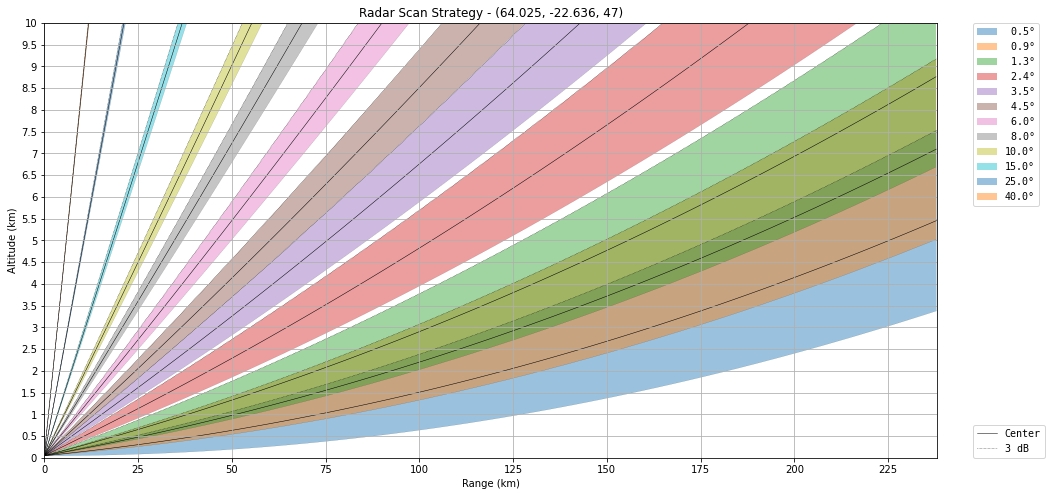
\includegraphics[width=\textwidth]{Pictures/Diagrams/Radar strategies/Strategy 1.png}
\caption{Radar strategy 1}
\label{fig:radarstrat1}
\end{figure}

\begin{figure}[H]
\centering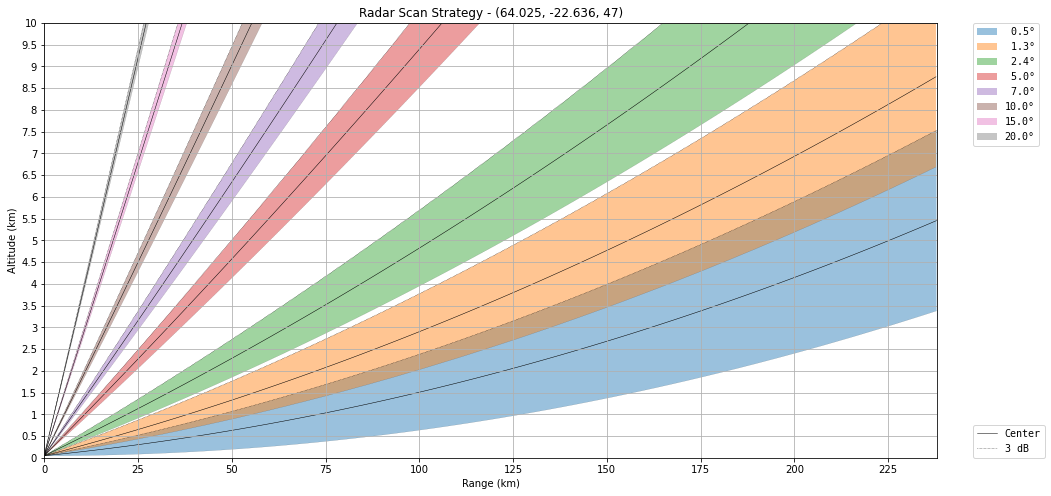
\includegraphics[width=\textwidth]{Pictures/Diagrams/Radar strategies/Strategy 3.png}
\caption{Radar strategy 3}
\label{fig:radarstrat3}
\end{figure}



\subsection{Numerical weather prediction data}
The numerical weather prediction data used in these experiments was provided by the Icelandic Meteorological office. The data included only the variable for the cumulative precipitation at 0m above ground, or in other words, estimated rainfall. The forecast has a forecast horizon of 66 hours, temporal frequency of 1 hour and spatial resolution of 2x2km and is updated every 6 hours. 

The accuracy of this forecast can be evaluated in and of itself by comparing rain-gauge observations with estimated rainfall. (this is something to do later) That can then be compared with the accuracy of radar estimated rainfall. 




\section{Data Processing}
This section will cover the specific methods used and the reasoning behind their usage.

% \subsection{Ensuring synchronization of data}
% A crucial part of data processing when working with time series, especially when these time series come from different datasets, where each dataset might vary in temporal frequency or might have missing values where the others don't. There are several kinds of datetime values that must be understood when processing data in order not to cheat in modelling as well as in order to ensure that all the correct data is made available to the model together in the correct order.

% Let's consider the case of a few different kinds of time series. 
% - One is a time series of observations $x_t$ such that at the time $t_k$, only observations from times $\leq t_k$ are available. 
% $x_t, t<t_k$
% - One is a time series of forecasts. We use the notation $\hat{x}_{T+h|T} $ to mean the value predicted for x, h time-steps into the future at time T. In this time series there might more more than one forecasts for a given time $t_a$, such as those made at times $t_{b}$ and $t_{c}$. These might be distinguished from one another by labeling them as ...

% An additional problem can pop up in these cases, one of RAM usage. To overcome this problem it is highly benefitial to utilize strides in numpy. This can let you use the data as if you have every possible sliding window including all the variables in both their past and future states in a single matrix without an overwhelming amount of RAM useage. 



\subsection{Temperature data}

\subsection{Temperature forecast data}


\subsection{Radar echo data}
Radar data processing is a ...

\cite{hess-17-863-2013}

One of the main considerations 


\section{Model}


\subsection{Drainage forecast from precipitation forecast}
Since 


\subsection{Precipitation forecasting models}
The first part of the complete model is the precipitation forecast itself. 



\subsection{Rainfall-runoff model}
The second part of the model is the rainfall-runoff model. The target variable for this model is the drainage flow at one or more pumping stations in the Reykjvaík drainage system. All parts of the drainage system in Reykjavík get input from one or more of the following sources: water used in for district heating, sewage and other wastewater, and rainfall-runoff. It should be highlighted that the district heating system in Iceland is not a closed loop and thus in most neighbourhoods will often enter the same route as rainfall water. That can be into the sewers or to a separate drainage system for non-sewage wastewater. 

If a model is supposed to forecast drainage flow it must have information about that predicts each of these sources. The first source, water for district heating use is relatively predictable in that mainly depends ambient outside temperature. The second source, sewage and other wastewater is relatively predictable in residential neighbourhoods, since they will follow very consistent patterns over the period of a day or a week. What remains to be predicted is the surface water from rainfall-runoff. 

% I think it's important to note here that getting the absolute best performance possible from this model wasn't the objective. The point of this subsection was a proof-of-concept for 1 or 2 kinds of models. The original thinking was that not too much focus would be put on this part because there was already going to be a lot of uncertainty in the feasibility of the overall model. 
The following experiment demonstrates the feasibility of modeling rainfall-runoff with the available data without incorporating future forecasting. The types of data sources considered in this experiment are: hourly average temperature data, raw 10 minute resolution rain-gauge data hourly and manually adjusted rain-gauge data. The target variables considered are hourly average flow measurements from several drainage stations. Before analysis and selection of variables, the entire year of 2020 was reserved for later testing purposes so as not to affect the decision process. 

To select the input and target variables several criteria were considered. Firstly, a dataset with an abundance of data was favored. All sensors with less than a year of data after 2020 had been removed were eliminated from consideration. For a visualization of the relative abundance of data was available for each target and input variable see figure \ref{fig:missingdata}.  Secondly, the wastewater treatment plants were eliminated as candidates since the size of these catchments means that spatial information becomes more important, which was not the objective of this demonstration. Thirdly the the system in question had to be a combined sewer to ensure that enough of an effect from rainfall-runoff could be observed for the demonstration. For this third factor, the correlation between the hourly accumulated rainfall and drainage flow was used as as a metric. To ensure that the the time-delay between maximal correlation of rainfall and drainage flow wouldn't affect the choice, the correlation between each rain-gauge-drainage flow meter pair was computed with up to 20 hours delay and the maximal correlation for each pair was used. The results of this can be seen in figure \ref{fig:maxcorrpairs}. 

\begin{figure}
\centering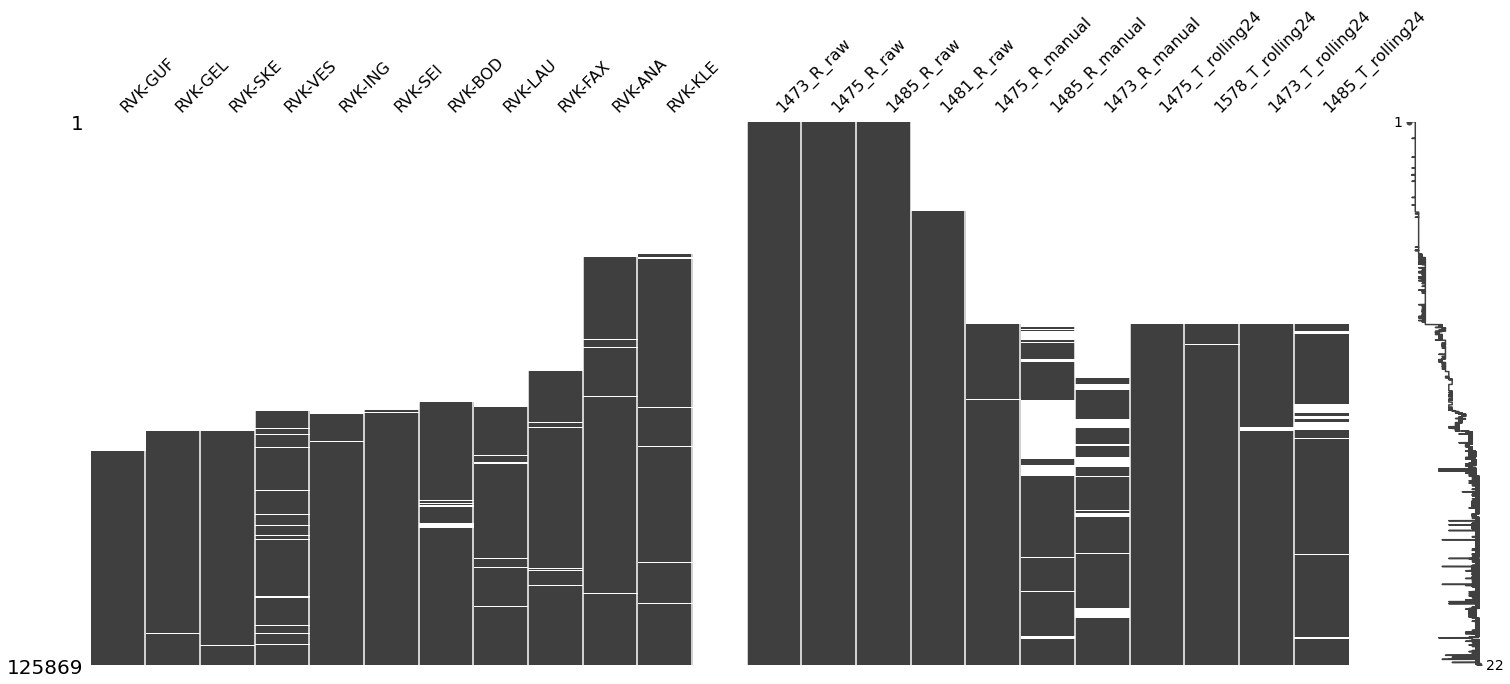
\includegraphics[width=\textwidth]{Pictures/Plots/missingdata.png}
\caption{Visualization of relative abundance of data for each of the target variables (left of the gap) and each of the input variables with data available since before 2019 (right of the gap)}
\label{fig:missingdata}
\end{figure}

\begin{figure}
\centering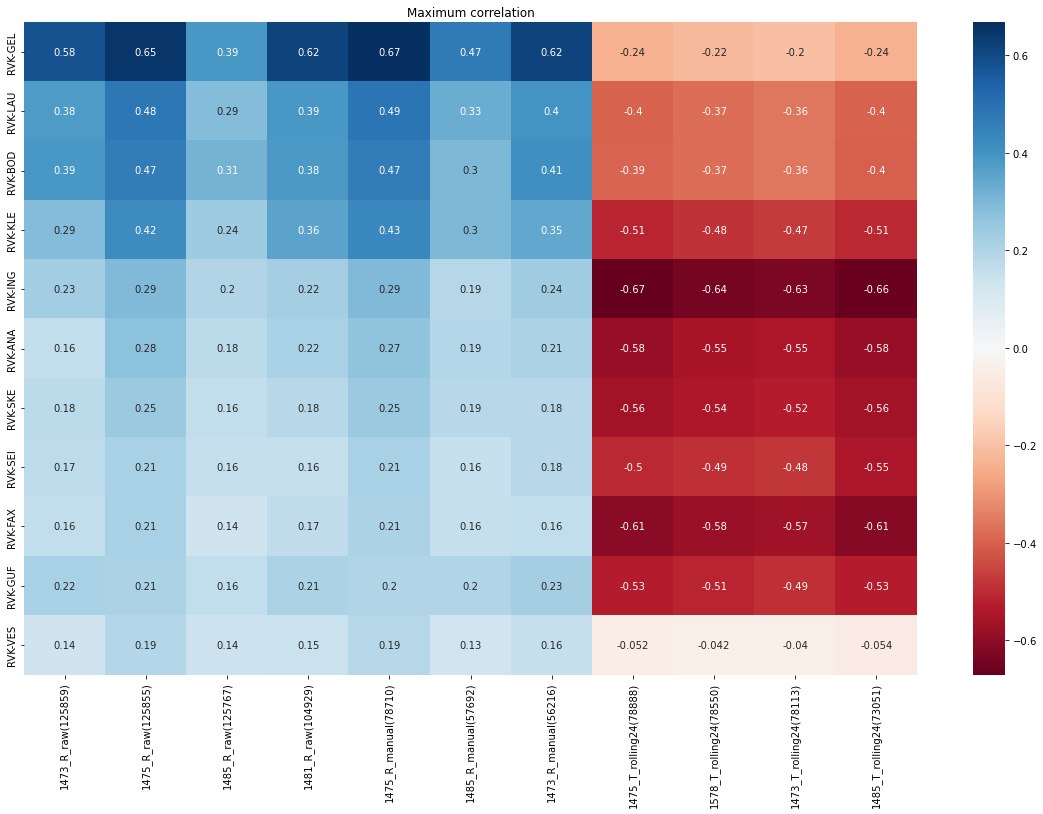
\includegraphics[width=\textwidth]{Pictures/Plots/max_corr_pairs.png}
\caption{Maximal correlation between hourly average drainage flow and hourly accumulated rainfall from each drainage flow sensor and rain-gauge not removed on the basis of a lack of data}
\label{fig:maxcorrpairs}
\end{figure}

For this experiment it was decided that two target variables be used: RVK-GEL and RVK-BOD. The input variables selected were both the rain-gauge and temperature data from sensor 1475 partly due to their high correlation with both variables and partly since the rain-gauge data was available as both raw and manually corrected.

%It might be good to include some further information about these drainage systems. For example I think both have quite a large industrial neighbourhoods and one is also very close to and responsible for the drainage of a 2x4 lane highway intersection and is also one of the older, if not the oldest parts of the drainage system in Reykjavík. 

Several variations of models and input data were tested. The exact description of these variations is explained 

It must be taken into consideration that not that all rain water that falls onto the surface immediately enters the drainage system, let alone flows all the way to the drainage flow meter on the way out of the pumping station. To account for this lag, the simplest solution is to include previous rainfall observations in addition to the most recent. 
% NOTE: if the increased dimensionality isn't an issue, since there is an abundance of training and testing data, it might be interesting to check if using the raw 10-minute rain-gauge values instead of the aggregated hourly cumulative rainfall gives a better result. Different time-scales aren't an issue if you just include all the extra data-points as more variables rather than more observations. 
How many previous observations it makes sense to include will be different for each pumping station. A rule of thumb in urban hydrology is that water travels at about one meter every second so it might make sense to allow for at least the distance across the catchment from the pumping station but in reality it can take much longer for water to flow to the end of the system, since it will often be delayed on the surface, in soil, on buildings or other geological features, not to mention the fact that precipitation in the form of snow will undoubtedly have a much longer delay than rain. 

Because of the uncertainty of this choice it was decided compare the performance of a linear regression model using a differing amount of lagged variables. % I'm really not so sure about this approach and I don't trust the fact that the first experiments (which I have yet to conduct more thoroughly) show that the performance just continues to improve unto something like 2 weeks back, which is 336 variables, and that as without regularization. 

Although the performance of the model did continue to marginally improve as more and more delayed variables were added, most of the improvements were for observations less than 12 hours old and after about 48 hours the performance has more or less completely plateaued. 


\section{Performance requirements of different drainage applications}
The main application considered the reduction combined sewer overflows (CSOs). To achieve this goal there are several approaches, most of which require building of additional infrastructure such as additional pumps, larger reservoir or other control mechanisms. For any solution that uses control mechanisms to reduce CSOs it is necessary to have some sort of input mechanisms 




\cite{ThorndahlRadar}